\documentclass[UTF8]{ctexart}
\usepackage{graphicx}
\usepackage{listings}
\lstset{showtabs=true}
\title{Computer Networking Lab 1: DNS Relay}
\author{PB22111620 Ai Chang}
\date{\today}
\begin{document}
\begin{sloppypar}
\maketitle

\section{代码结构与作用}
    \subsection{代码结构总览}
        代码整体结构及作用如下
            \begin{itemize}
                \item def config(path)--用于从 example.txt 中得到 domain-ip 的
                    对应关系, 并构造字典
                \item class query\_part--用于处理问题节, 提取其内容/将提取出的内容打包
                    \begin{itemize}
                        \item unpack(self, data)--提取 Qname, Qtype, Qclass
                        \item pack(self)--将上述内容打包
                    \end{itemize}
                \item class message--处理整个报文段
                    \begin{itemize}
                        \item unpack(self, data)--将报文头部解封装, 若报文是查询
                            报文, 则进一步解析问题节
                        \item r\_pack(self, ip)--根据得到的 ip 和查询报文内容生成
                            回复报文
                    \end{itemize}
                \item relay\_server--总揽全局, 统筹收到报文后需要做的各项工作
                    \begin{itemize}
                        \item process(self, data, addr)--处理报文
                        \item run(self)--用于循环接受 DNS 报文
                    \end{itemize}
            \end{itemize}
    \subsection{关键功能实现}
        \begin{enumerate}
            \item 收到报文后的处理逻辑
                \begin{lstlisting}[language=Python,
                    frame=single]
def process(self, data, addr):
start_time = time()
m = message(data)
if m.qr == 0:
    name = m.query.name

    if name in self.config and m.query.type == 1:
        ip = self.config[name]
        if ip == "0.0.0.0":
            response = m.r_pack(ip)
            self.s.sendto(response, addr)
            print('query to %+50s'%name, 'handled
                 as      intercept, takes','%fs'
                 %(time()-start_time),sep='\t')
        else:
            response = m.r_pack(ip)
            self.s.sendto(response, addr)
            print('query to %+50s'%name, 'handled
                 as local resolved, takes','%fs'
                 %(time()-start_time),sep='\t')
    else:
        self.s.sendto(data, self.nameserver)
        self.transaction[m.id]=(addr,name,time())
else:
    if m.id in self.transaction:
        target_addr, name, start_time =
             self.transaction[m.id]
        self.s.sendto(data, target_addr)
        print('query to %+50s'%name, 'handled
             as          relay, takes','%fs'
             %(time()-start_time),sep='\t')
        del self.transaction[m.id]
                \end{lstlisting}
                收到报文后, 记录开始时间用于后面计算处理报文用时, 并调用
                message(data) 分解报文. 若该报文是查询报文, 查询该域名
                是否在配置中, 若在, 判断该报文是否有意义, 若有, 则本地处
                理并发送答复报文, 否则直接阻断, 然后发送答复报文. 若该域
                名不在配置中, 发送给指定的公共 DNS server 处理, 并记录
                该报文信息, 后面收到 DNS server 的答复时匹配. 若该报文
                不是查询报文, 可能是来自公共 DNS server 的答复, 与记录
                中的报文做匹配, 若匹配成功, 则将该报文转发给请求端.
            \item 提取并打包问题节
                \begin{lstlisting}[language=Python,
                    frame=single]
def unpack(self, data):
    self.name = []
    i = 0
    length = 0
    label = ''
    while True:
        d = data[i]
        if length == 0:
            self.name.append(label)
            label = ''
            if d == 0:
                break
            else:
                length = d
        else:
            label += chr(d)
            length -= 1
        i += 1
    self.name = '.'.join(self.name[1:])
    self.type, self.classify = struct.unpack
        ('>HH', data[i + 1:i + 5])
    self.idx = i + 5
def pack(self):
    labels = self.name.split('.')
    data = bytearray()
    for label in labels:
        data.append(len(label))
        data.extend(label.encode('utf-8'))
    data.append(0)
    data.extend(struct.pack('>HH',
         self.type, self.classify))
    return data
                \end{lstlisting}
                其中 unpack 用于提取问题节的内容, 因为域名长度是不固定的, 所以
                需要用 length 记录当前域名的大小, 从而提取相应大小的字符. 解析
                域名之后, 因为不需要进行边界填充对齐, 故 Qtype, Qclass 紧跟在
                Qname 之后四位, 用 data[i+1:i+5] 即可提取出来, 同时用 idx
                记录下问题节的大小, 在生成答复节时使用

                pack 用于打包问题节, 通过将域名根据 '.' 分组, 依次将各部分存入
                data, 最后将 type, classify 存入 data.(实际上, 我并不是很清楚为什么要将问题节打包, 而不是直接使用传入的报文)
            \item 生成应答报文
                \begin{lstlisting}[language=Python,
                    frame=single]
def r_pack(self, ip):
timetolive = 200
datalength = 4
s = ip.split('.')
response_header = struct.pack('>HHHHHH',
     self.id, self.flags, self.quests, 
     self.answers, self.author, self.addition)
question = self.query.pack()
answer = question[:self.query.idx]
answer += struct.pack('>HHHH', 1, 1, timetolive,
     datalength)
answer += struct.pack('BBBB', int(s[0]),
     int(s[1]), int(s[2]), int(s[3]))
return response_header + question + answer
                \end{lstlisting}
                应答报文 = 头部 + 问题 + 答复, 我们生成应答报文时也根据这三部分
                来实现. 首先是头部, 头部包括 identification, flags,
                 questions, answers, authority, addition, 各部分都在
                 unpack 中得到, 直接填入即可得到 response\_header; 问题节
                部分直接调用 query\_part 的 pack 得到; 答复节包含 Qname,
                 Qtype, Qclass, TTL, Rdatalength, Rdata, 前面三部分由
                 question 即可得到, TTL, datalength 是定值, 直接填入.
                 Rdata 部分只需将 ip 根据 '.' 分为四部分, 依次填入即可
            \item 并发查询
                \begin{lstlisting}[language=Python,
                    frame=single]
def run(self):
while True:
    try:
        data, addr = self.s.recvfrom(1024)
        threading.Thread(target=self.process,
             args=(data, addr)).start()
    except Exception:
        pass
                \end{lstlisting}
                该部分已经由代码框架实现
        \end{enumerate}
\section{实验结果}
    \subsection{程序输出}
        \begin{figure}[h]
            \centering
            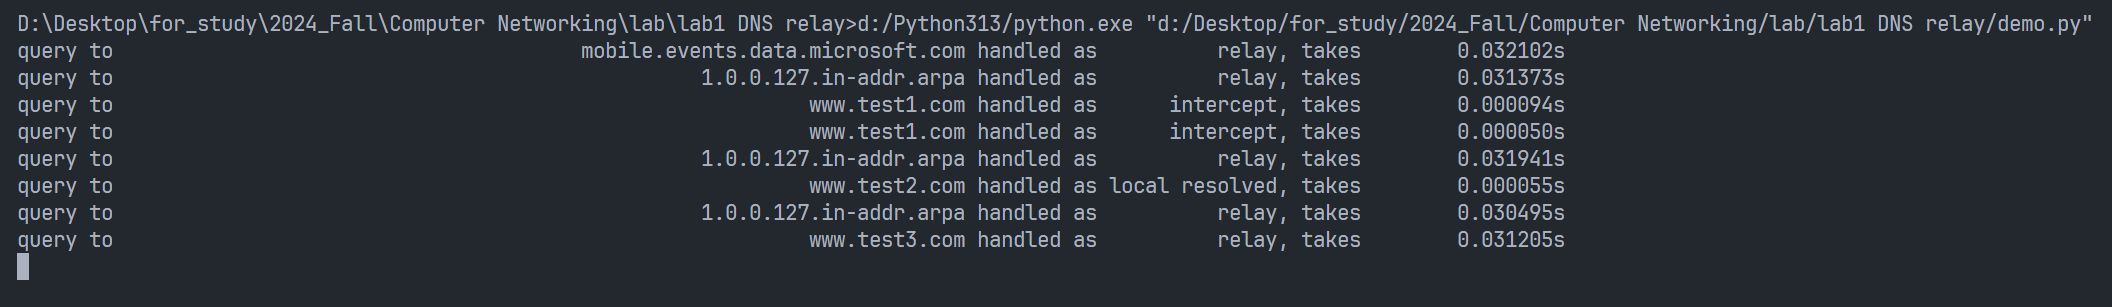
\includegraphics[scale=0.2]{resources/programme_output1.png}
        \end{figure}
        程序输出结果如上图所示, 对于配置中的 www.test1.com,
        www.test2.com, 程序分别识别为 intercept,
        local resolved. 而配置中没有的 test3, 程序
        对其进行了 relay. 同时可以发现, 查找配置中存在的
        域名所需时间要短得多, 这与 cache 的工作原理一致.
    \subsection{nslookup}
        \begin{figure}[h]
            \centering
            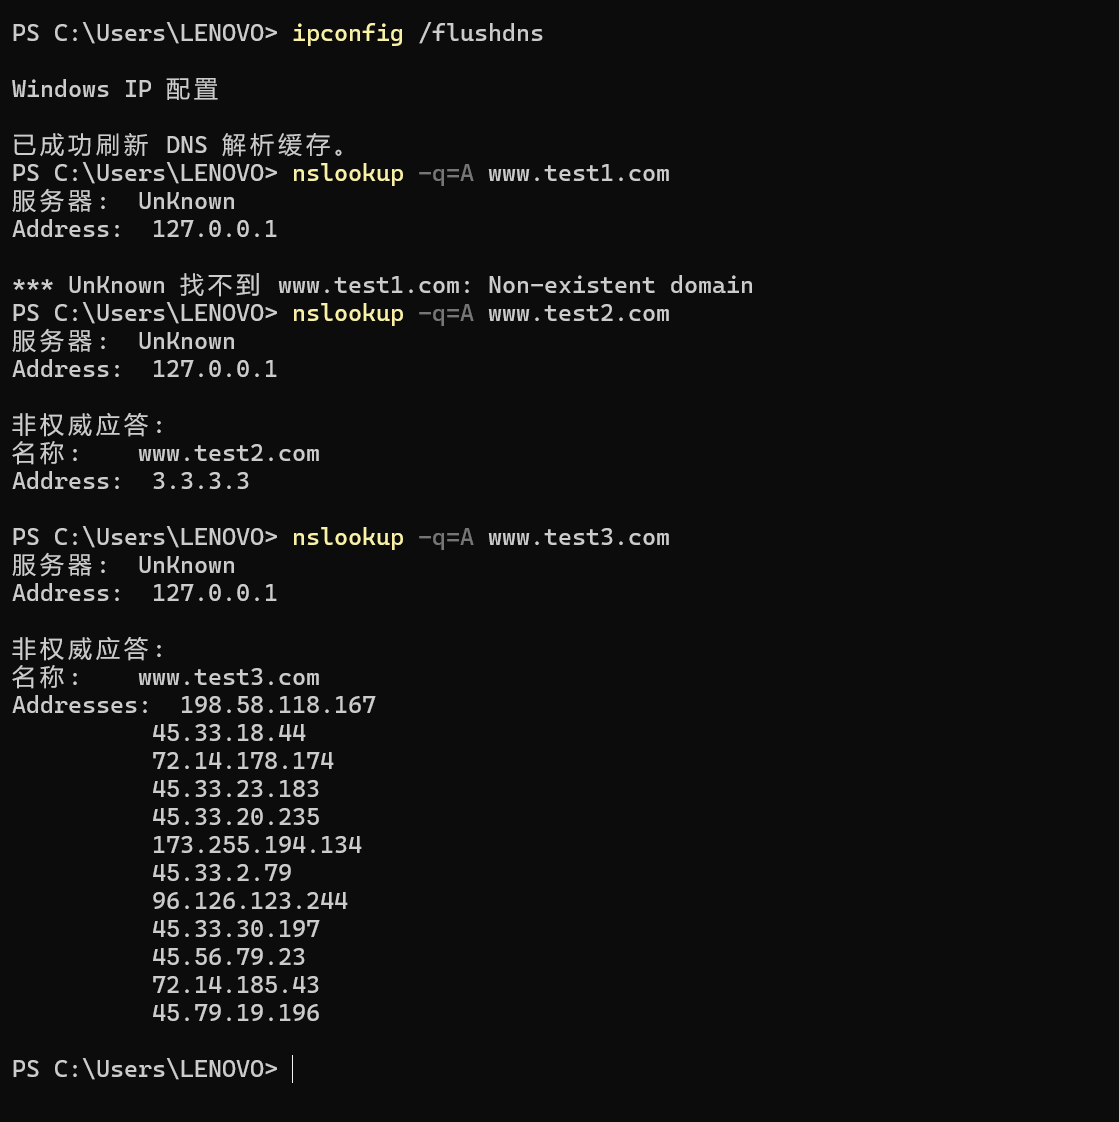
\includegraphics[scale=0.25]{resources/terminal_output1.png}
        \end{figure}
        在终端中进行 nslookup 查询后结果如上图所示, 与助教
        提供的样例一致(为提高辨识度, 已在 example.txt
         中将 www.test2.com 的 ip 改为 3.3.3.3)
    \subsection{浏览器测试}
        \begin{figure}[h]
            \centering
            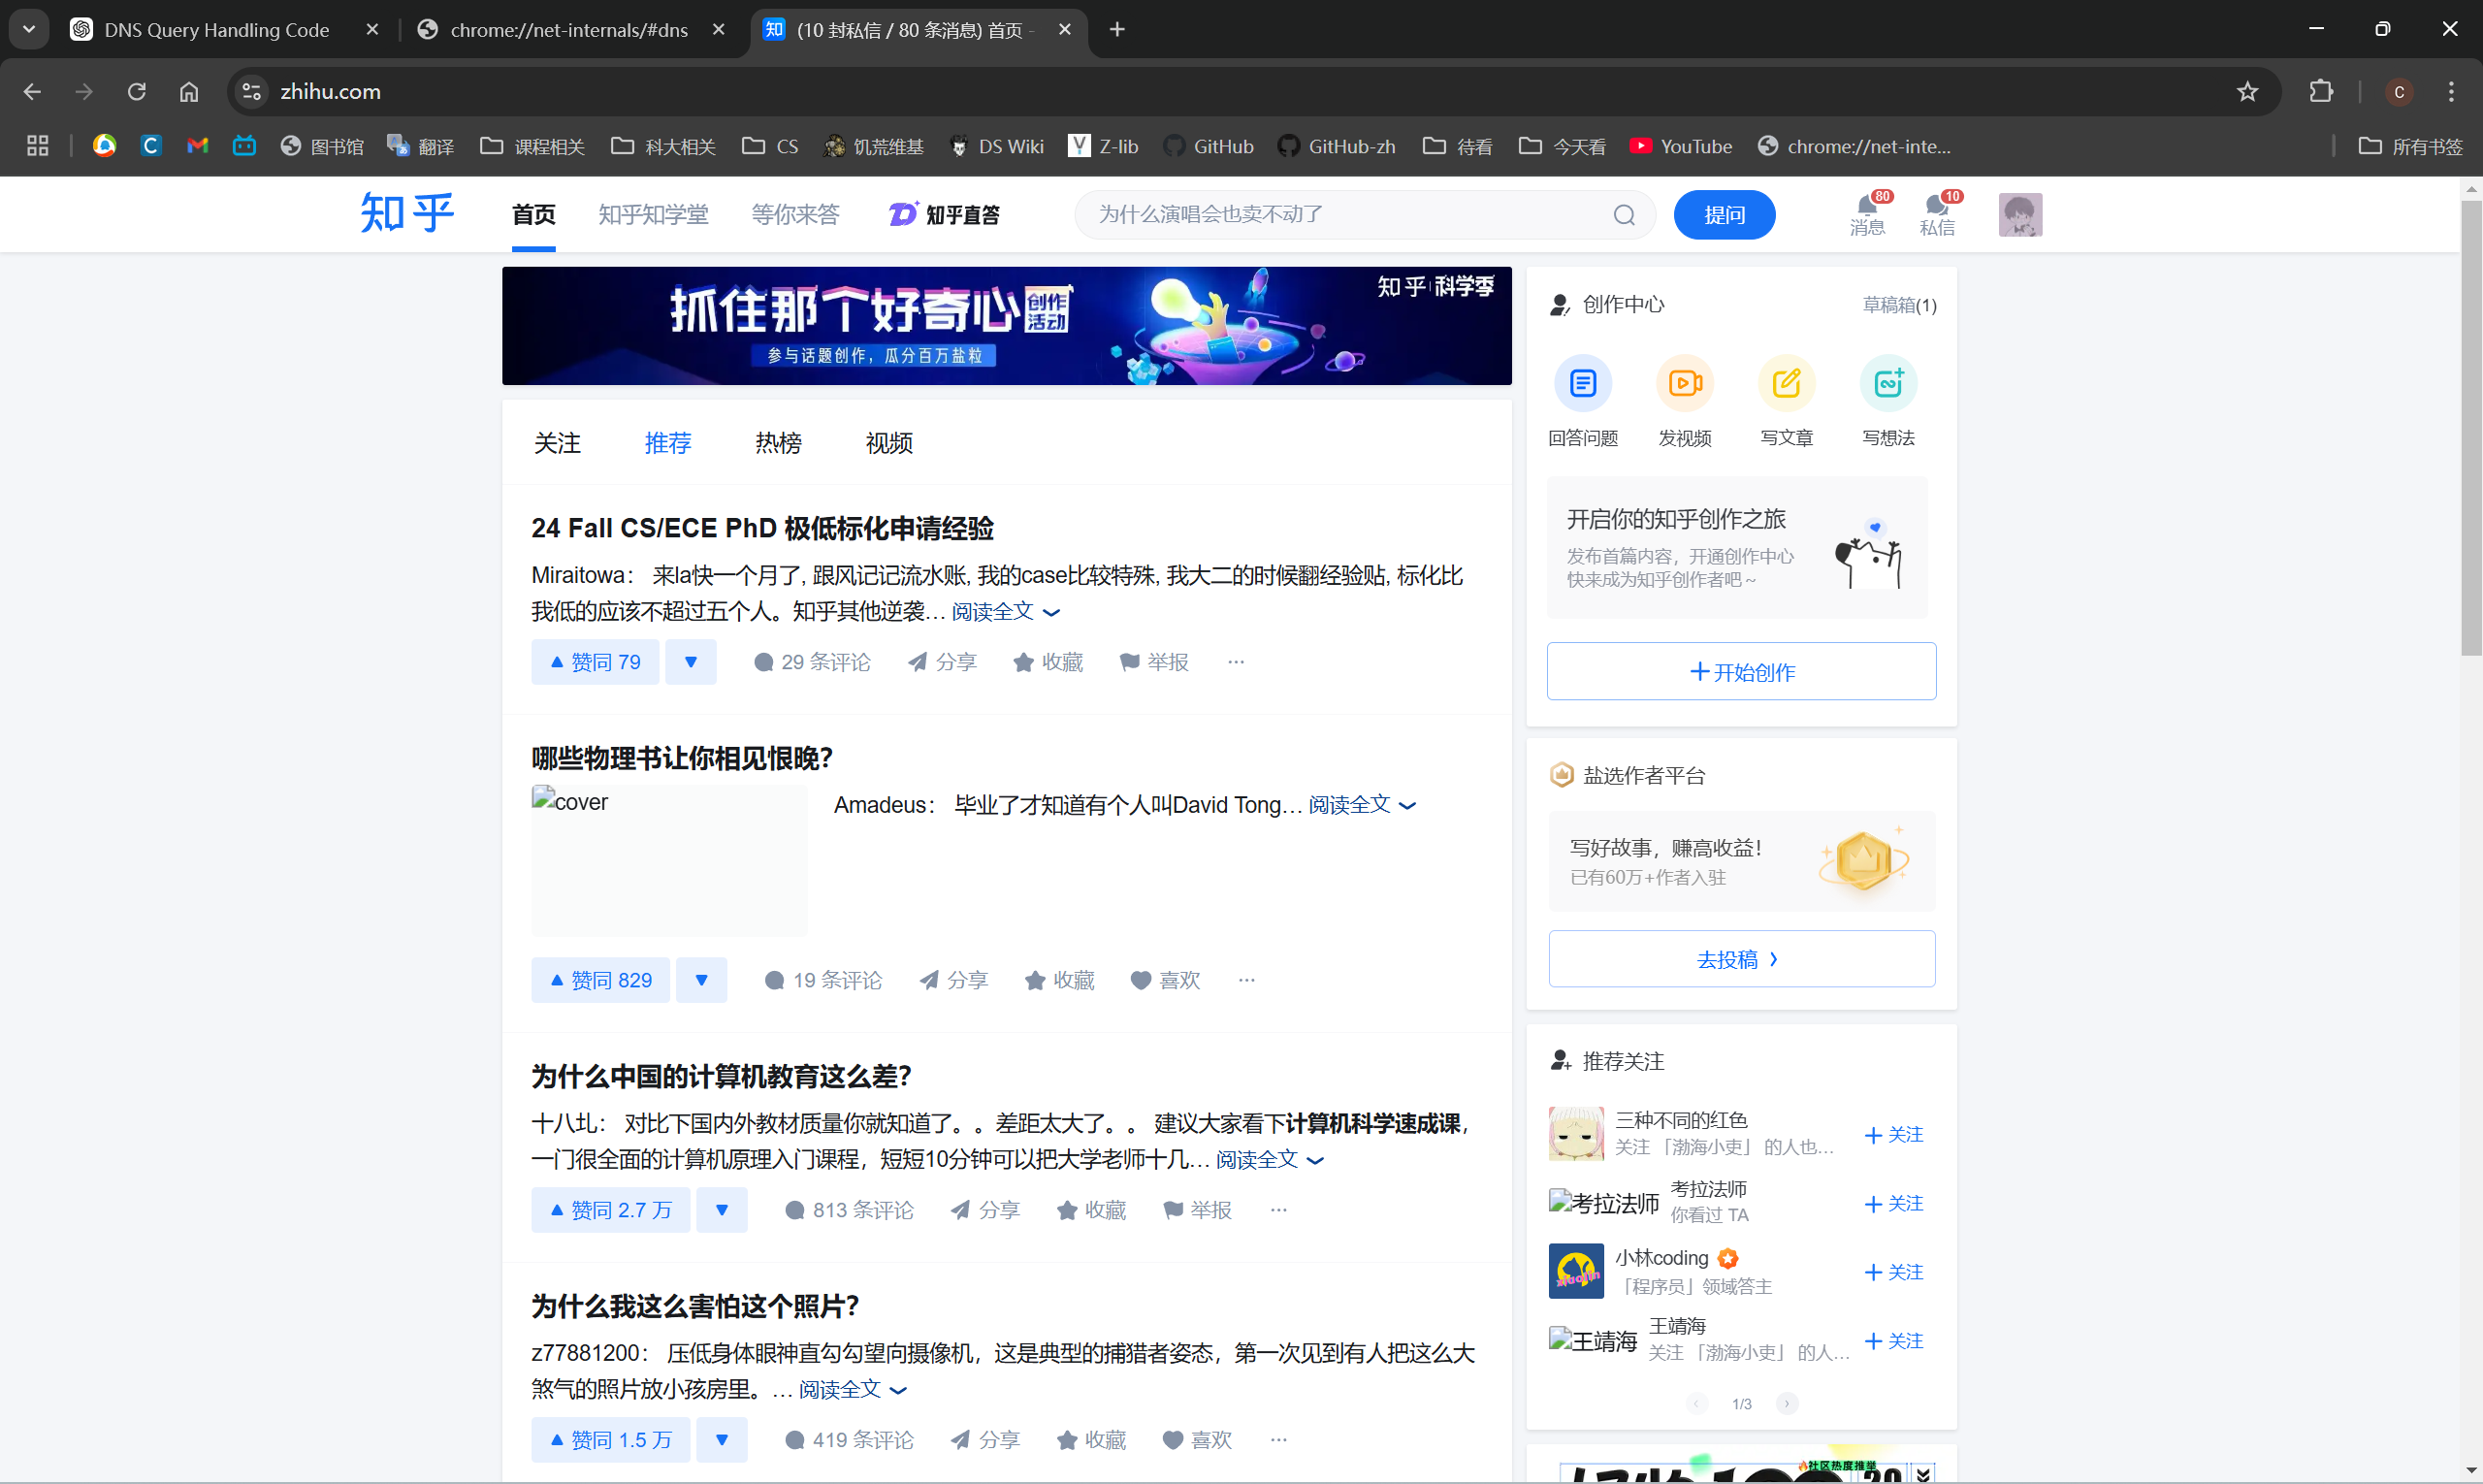
\includegraphics[scale=0.15]{resources/zhihu_output.png}
        \end{figure}
        浏览器测试结果如下图所示, 通过 F12 检查网页的
         resources, 发现只有部分图片被拦截, 不是很清楚
        其中的原因


\vspace*{7em}


\section{其他}
    本次实验中遇到了诸多问题, 在此写一下完成后的体验.
    \begin{enumerate}
        \item 实验整体还是学到了不少东西
        \item 之前只在写大物实验时自学了一点 python 用于处理数据,
         这次实验中理解实验框架, 使用 python 实现功能比较困难.
        \item 实验过程中遇到了 bug, 即程序正常运行而终端无法输出
        正确结果. 多次尝试无果后, 在助教的提示下将我生成的答复报文与
        标准答复报文对比, 最终发现是对实验文档理解有误, 没有使用 "DNS
         报文压缩" 功能, 导致了报文中出现了重复字段, 终端无法正常识别.
         在修改了相应代码后, 得到了想要的结果.
    \end{enumerate}
\end{sloppypar}
\end{document}